Abbildung \ref{fig:aufbau} zeigt den prinzipiellen Aufbau des Versuchs.
\begin{figure}
  \centering
  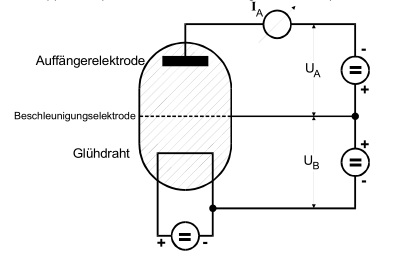
\includegraphics[width=0.7\textwidth]{bilder/aufbau.jpg}
  \caption{Prinzipieller Aufbau des Franck-Hertz-Versuchs \cite{601}.}
  \label{fig:aufbau}
\end{figure}
Der Aufbau besteht aus einem Glasrohr, welches mit Hg-Dampf gefüllt ist,
sowie einem Heizfaden, einer Beschleunigungs- und einer Auffängerelektrode
die ebenfalls im Glasrohr untergebracht sind.
Das Glasrohr selbst befindet sich einem heizbaren Blechgehäuse, dessen
Innentemperatur $\su{T}$ mit einem elektrischen Temperaturreglers konstant
gehalten wird. Die Temperatur wird mit einem Thermometer abgelesen.

Der Glühfaden wird durch ein seperates Konstantspannungsgerät versorgt, welches
sich präzise einstellen lässt. Beschleunigungs- und Bremsspannung werden von
zwei elektronischen Geräten geliefert, deren Ausgangsspannung sich
zeitproportional ändern kann. Der Auffängerstrom wird auf seiner geringen Größe
mit einem Picoamperemeter gemessen. Hierbei handelt es sich um einen
Gleichstromverstärker mit eingebautem Amperemeter, dessen Ausschlag proportional
zum Eingangsstrom ist. Die Franck-Hertz-Kurve wird mit einem XY-Schreiber
aufgezeichnet, bei dem am X-Eingang die Beschleunigerspannung und am Y-Eingang
eine Spannung, die proportional zum Auffängerstrom ist, angelegt wird. Diese
Spannung wird vom Picoamperemeter geliefert.

Um die Energieverteilung der
Elektronen zu messen, wird bei konstanter Beschleunigerspannung $\su{U_B}$ die
Gegenspannung an der Auffängerelektrode von 0 ausgehend bis zu einem Maximalwert
erhöht. Der Auffängerstrom $\su{I_A}$ wird dabei in Abhängigkeit von $\su{U_A}$
vom XY-Schreiber aufgezeichnet.

Die Ionisierungsspannung $\su{U_{ion}}$ von Quecksilber wird gemessen, indem eine
konstante negative Spannung von etwa $30\Volt$ an die Auffängerelektrode angelegt
wird, sodass alle erzeugten Ionen auf der Elektrode landen. Die Elektronen werden
dabei jedoch zurückgehalten.
Nun wird $\su{U_B}$ allmählich erhöht und $\su{I_A}$ gemessen. Der Auffängerstrom
steigt stark an, wenn die Elektronen eine Energie erreichen, die sie zur
Ionisierung befähigen.
Die verwendete Schaltung für die einzelnen Messungen ist in Abbildung \ref{fig:schalt}
dargestellt.
\begin{figure}
  \centering
  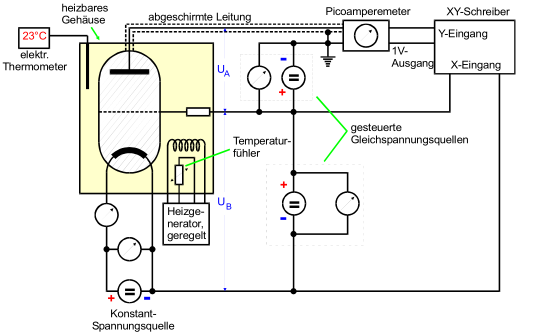
\includegraphics[width=0.7\textwidth]{bilder/schalt.jpg}
  \caption{Schaltung zur Aufnahme einer Franck-Hertz-Kurve \cite{601}.}
  \label{fig:schalt}
\end{figure}
Durch Erhitzen des Gehäuses wird der benötigte Hg-Dampfdruck eingestellt, sodass
der Ausgangsstrom einen Maximalwert zwischen $2.1\Amp$ und $2.2\Amp$ erreicht.
Wenn die gewünschte Temperatur erreicht ist, wird Regelknopf soweit zurück
gedreht, dass der Ausgangsstrom einen Minimalwert von etwa $1.2\Amp$ erreicht.
Um eine Franck-Hertz-Kurve aufnehmen zu können, muss die Heizleistung des
Glühfadens heruntergeregelt werden, sodass der maximale Auffängerstrom für die
Spannung $\su{U_B}\approx60\Volt$ einen Wert zwischen $1\nA$ und $3\nA$ erreicht.

Um den XY-Schreiber zu justieren werden die Nullpunkte beider Messskalen in die
linke untere Ecke des Diagramms gelegt. An den Eingängen wird hierbei kein
Signal angelegt. Die Empfindlichkeiten der beidern Eingänge werden geeignet
eingestellt. Hierfür wird zunächst ein unempfindlicer Bereich gewählt, damit
die Feder bei einem zu hohen Signal nicht an den Anschlag getrieben wird, was
eine überlastung des Antriebsmotors zur Folge hat. Die Empfindlichkeit wird nun
weiter gesteigert, dass für den Y-Kanal bei einem Strom $\su{I_A}\approx3\nA$
der Ausschlag des Schreibers noch etwas unter dem Vollausschlag liegt. Die
X-Achse muss, im Gegensatz zur y-Achse, in Volt geeicht werden. Dazu wird
die X-Empfindlichkeit so eingestellt, dass für die Maximalspannung eine volle
Auslenkung in X-Richtung erreicht wird.
